\section{Literature Review}\label{sec:literature}

\subsection{Scope and Method}

A targeted search of Google Scholar, IEEE Xplore, MDPI, and ScienceDirect was performed across six themes -- visual-analytics design and evaluation, visual analytics for emergency management, spatial analysis of incident data, fire-station optimisation, London-specific work, and predictive analytics for emergency events. Thirty papers spanning 1974--2024 were read in depth; the review distinguishes foundational design references (Shneiderman's mantra; Munzner's nested model; Church and ReVelle's covering-location formulation) from contemporaneous comparable work (Park et al.\ on Seoul, Bispo et al.\ on Aveiro, Taylor on London 2012--2014) and from the uncertainty-visualisation, modern-dashboard, and distributive-justice literatures that frame the dashboard's core design decisions. Each cited paper was checked against its primary source where the full text was accessible, rather than against secondary summaries; for older foundational works where full text was not accessible, the relevant formulations were cross-checked against publisher metadata and subsequent peer-reviewed uses. Where common framings of the literature diverge from the actual published work, the prose below reflects the latter.

\subsection{Visual Analytics: Design Principles, Tools, and Emergency Applications}\label{sec:lit-va}

Dashboard design for spatial-event data follows Shneiderman's Visual Information Seeking Mantra -- ``overview first, zoom and filter, then details-on-demand'' \cite{shneiderman1996} -- operationalised through a task-by-data-type taxonomy of seven tasks (Overview, Zoom, Filter, Details-on-demand, Relate, History, Extract). The dashboard's interaction repertoire is further organised around the user-intent categories of Yi et al.\ \cite{yi2007}: Filter (borough/year/category selection), Connect (brushing across linked map and time-series), Explore (map pan/zoom), and Abstract/Elaborate (hover tooltips). At the implementation layer, the dashboard adopts the declarative-visualisation paradigm \cite{heer2010,bostock2011}, which separates visual specification from execution by binding data to W3C DOM elements (SVG/HTML) via the \texttt{enter/update/exit} pattern; D3.js \cite{bostock2011} is the web-native realisation of that paradigm. Munzner's nested design model \cite{munzner2009}, elaborated in book-length form in \emph{Visualization Analysis and Design} \cite{munzner2014}, provides the cross-cutting validation framework: characterise task and data first, then choose operations and data types, then design encodings and interactions, then implement -- because the model gives an explicit place to record decisions at each layer and makes it harder to mask a poorly-defined task with good-looking visuals. Section~4.6 utilizes the seven-scenario evaluation taxonomy of Lam et al.\ \cite{lam2011} to organize the evaluation strands. This taxonomy surveys 850 InfoVis papers and consolidates evaluation goals into scenarios spanning user experience, performance, and visual data reasoning.

Where Shneiderman's mantra frames an analyst's interaction with arbitrary data, more recent work argues that \emph{dashboards} form a distinct sub-class with their own design space. Sarikaya et al.\ \cite{sarikaya2018} structure that space along four axes -- purpose, audience, visual-and-interactive features, and data semantics -- and derive seven dashboard genres from a corpus of 83 in-the-wild examples. Bach et al.\ \cite{bach2023patterns} extend the corpus to 144 dashboards and consolidate 42 design patterns across content, composition, and interaction, articulating a four-parameter trade-off between abstraction, screenspace, pagination, and interaction (any reduction along one parameter forces an increase along another). The proposed LFB dashboard sits at the intersection of the operational-decision-making and public-communication genres of \cite{sarikaya2018}, and instantiates the analytic genre of \cite{bach2023patterns} with a stratified page layout, hierarchical drill-down (London $\to$ borough $\to$ station-related context), and a schematic-spatial layout for comparing linked borough evidence.

Emergency-management reviews find that maps and dashboard composites dominate, but most systems remain post-hoc analytical tools~\cite{dusse2016,marbouti2016}. The closest architectural exemplar is Reinert et al.'s PanViz~2.0~\cite{panviz2020}: a Flask/React application combining controls, a county choropleth, and aligned temporal panels (Figure~\ref{fig:panviz-interface}). This project borrows that linked control--map--time structure but changes the analytical contract. PanViz simulates epidemic spread under user-set parameters; the LFB artefact displays observed borough evidence, adds distribution and ranking views, and exposes denominator and coordinate-completeness caveats. The comparison therefore supports the interface architecture, not a claim that the two systems answer the same question.

\begin{figure}[H]
\centering
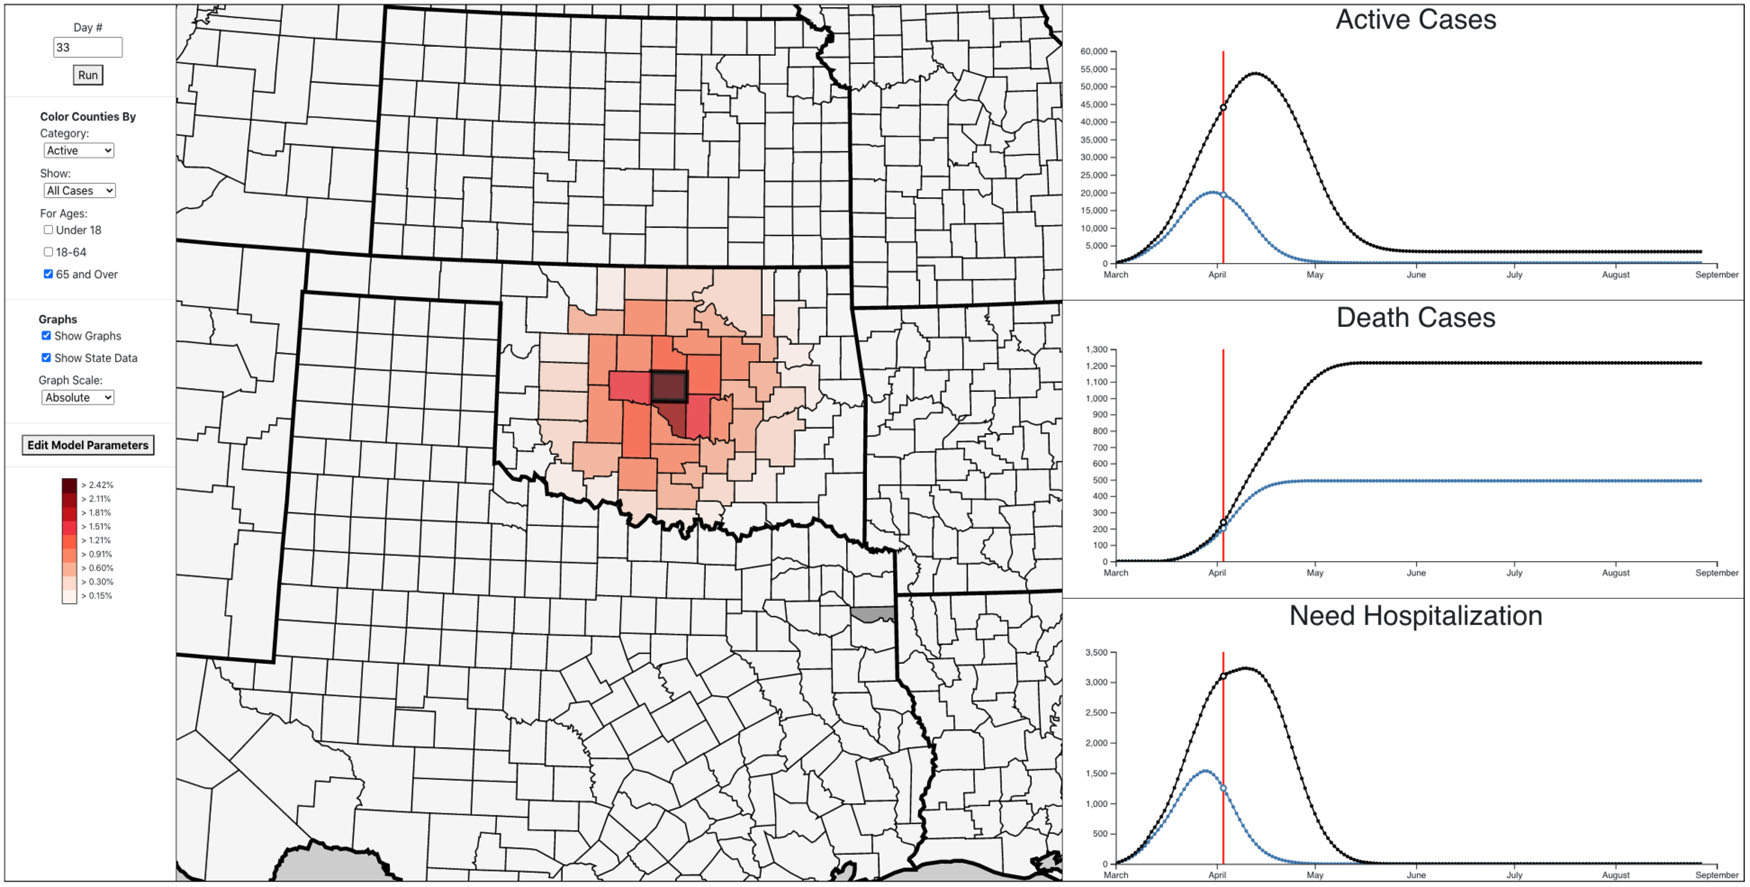
\includegraphics[width=\textwidth]{figures/literature/fig_panviz2_interface_reproduced.png}
\caption{PanViz~2.0 interface: model controls, county map, and aligned temporal outputs. Source: Reinert et al.~\cite[Fig.~1]{panviz2020}, \textcopyright{} 2020 IEEE. Reproduced without alteration.}
\label{fig:panviz-interface}
\end{figure}

Beyond these exemplars, alternative input modalities have been explored: Imran et al.'s survey \cite{imran2015} catalogues social-media-driven situation awareness during mass emergencies, and AR-augmented spatial communication \cite{sharmaAR2023} extends the modality further. These alternative streams are noted for completeness; their applicability to a planning-focused LFB dashboard, which works from structured incident records rather than user-generated content, is peripheral.

\subsection{Uncertainty-Aware Visualisation}\label{sec:lit-uncertainty}

The project's framing as an \emph{uncertainty-aware} dashboard is grounded in three complementary literatures, none of which has previously been brought to bear on emergency-services performance data. From the visualisation-design side, Hullman, Resnick and Adar \cite{hullman2015hops} show in a 288-subject controlled experiment that static error bars and violin plots produce mean absolute errors three-to-four times larger than animated Hypothetical Outcome Plots on probabilistic-comparison tasks (estimating $\Pr(B>A)$ across pairs of distributions); reliance on point estimates and binary-coverage error bars therefore systematically misleads non-expert readers, the precise audience for a public-facing performance dashboard. From the cartographic side, MacEachren et al.\ \cite{maceachren2012} establish empirically that only \emph{fuzziness}, \emph{location offset}, and \emph{colour value} are intuitively read as uncertainty by GIScience-literate users, while colour saturation -- the variable most commonly assumed to encode confidence -- is not; encoding the LFB dataset's geocoding incompleteness (only 37.9\% of records carry valid coordinates) therefore demands fuzziness or value ramps rather than the saturation channel default. From the cognitive-science side, Padilla, Creem-Regehr, Hegarty and Stefanucci \cite{padilla2018} embed uncertainty visualisation in dual-process decision theory: visual-spatial biases such as the deterministic-construal error (e.g.\ misreading error bars as absolute high/low bounds, or reading the Cone of Uncertainty as physical growth) arise during Type-1 bottom-up attention and resist correction even when a key is provided. The implication is that the LFB dashboard cannot rely on legends or footnotes to discharge its uncertainty-awareness; the encodings themselves must be Type-1-readable. The current implementation enacts a narrower first iteration: median-to-p95 ranges, explicit denominator text, and precise-coordinate coverage fields. Full quantile dotplots, map fuzziness, and natural-frequency tooltip phrasing remain second-iteration items rather than completed results.

\begin{figure}[H]
\centering
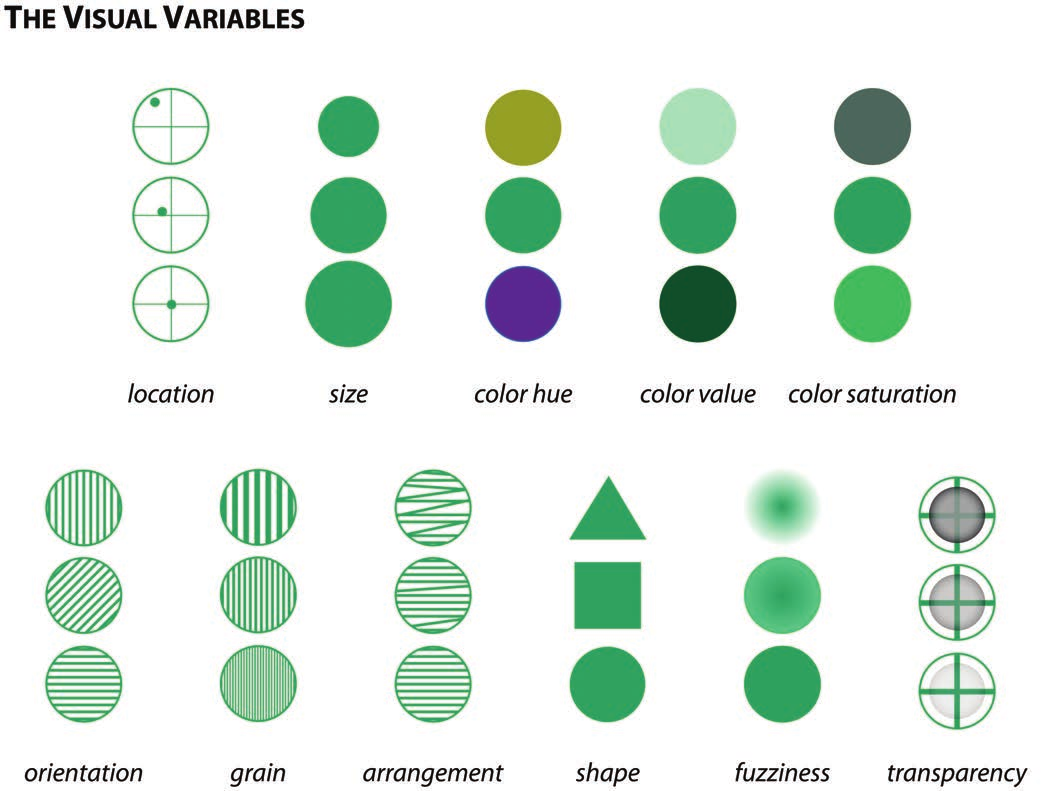
\includegraphics[width=0.82\textwidth]{figures/literature/fig_maceachren_visual_variables_reproduced.png}
\caption{Eleven visual variables considered by MacEachren et al.\ for ordinal uncertainty, including location, colour value, colour saturation, and fuzziness. Source: MacEachren et al.~\cite[Fig.~1]{maceachren2012}, authors' prepublication manuscript. Reproduced without alteration.}
\label{fig:maceachren-visual-variables}
\end{figure}

\subsection{Spatial Analysis of Emergency and Fire Incidents}\label{sec:lit-spatial}

\textbf{Seoul grid evidence:} The methodologically closest comparable study at comparable scale is Park, Kwon and Azam's GIS-based spatial analysis of Seoul fire-emergency response \cite{seoul2024}. After filtering 846{,}384 raw 2017--2022 Seoul rescue reports, they retain 56{,}514 life-saving cases on a 500\,m\,$\times$\,500\,m grid covering Seoul (3{,}227 grids). The analytic threshold is 5 minutes from dispatch to scene, used as the operational proxy for the broader ``golden time'' concept. They report Global Moran's $I = 0.45$ ($p<0.001$) for the full incident distribution and 0.57 for the $>$5-minute subset, and use Local Moran's I (LISA) to localise hotspots. Three findings inform this project: (i) the $>$5-minute subset is more spatially clustered than the full incident distribution, indicating that response equity is geographically structured beyond what raw incident density would predict; (ii) the Seoul mean grid-to-nearest-station straight-line distance of 1.34\,km masks district-level variation, with Songpa-gu, Gwanak-gu and the area south of the Han River exceeding 1.45\,km, and traffic volume alone does not explain the $>$5-minute clustering, attributing it instead to station-spacing gaps; (iii) the proxy of ``nearest-station'' distance is computed straight-line, which supports using transparent straight-line station-address proximity as context while still stopping short of a network-routing model. The 5-minute Seoul threshold is the methodological analogue of the LFB 6-minute first-pump target. Two limitations of Park et al.\ shape the present design: their grid-level coverage analysis depends on geocoded arrival points (LFB has only 37.9\% geocoded), and their proximal-station definition uses straight-line rather than road-network distance.

\textbf{Taylor closure cohort:} Taylor's spatial-survival analysis of LFB dwelling-fire response times~\cite{spatial2015} fits separate 2012--2014 proportional-hazards models with harmonic diurnal terms and spatially correlated frailties on a 500\,m grid. Adjusted relative risk falls below 1 during 3am--7am and 11am--6pm, with a trough near 0.7 at 5am, showing that raw temporal aggregation can conceal spatially conditioned effects. The present dashboard exposes hour and day slices but does not reproduce Taylor's spatial adjustment, so the study is a caution and historical benchmark rather than an implemented algorithm. Of ten stations closed in 2014, eight had surrounding grid cells with $\geq$80\% posterior probability that P(response\,$>$\,360s) rose by at least 0.1 relative to both prior years; Bow and Clerkenwell were not similarly affected. The comparison in \S6 is therefore descriptive and explicitly limited by Taylor's dwelling-fire-only scope and finer granularity.

\begin{figure}[p]
\centering
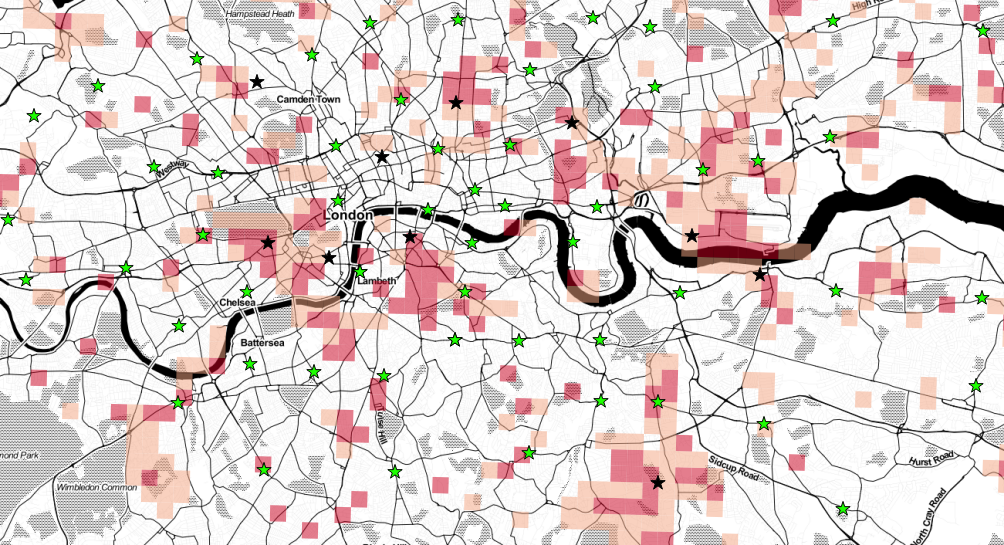
\includegraphics[width=0.74\textwidth]{figures/literature/fig_taylor_probability_2014_vs_2012.png}\\[-0.35em]
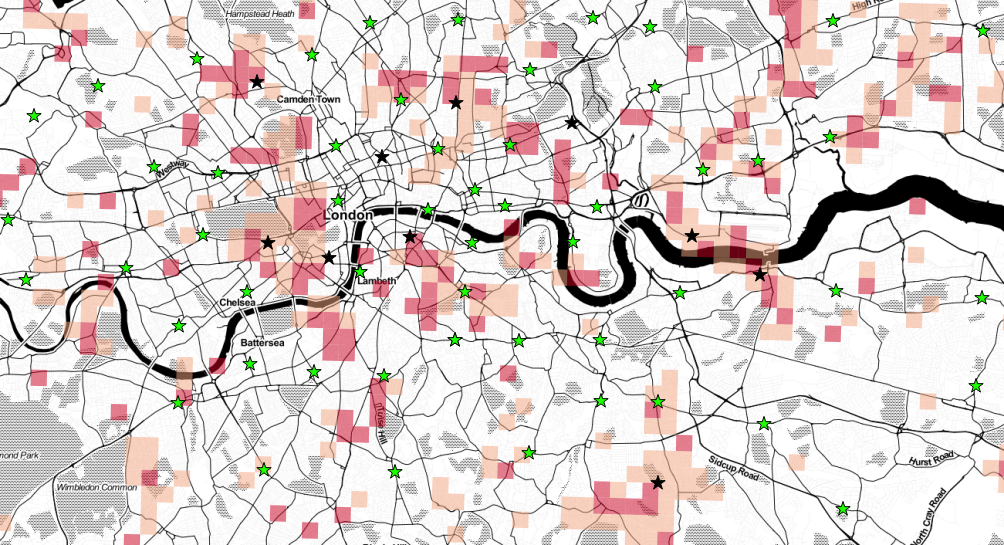
\includegraphics[width=0.74\textwidth]{figures/literature/fig_taylor_probability_2014_vs_2013.png}\\[-0.35em]
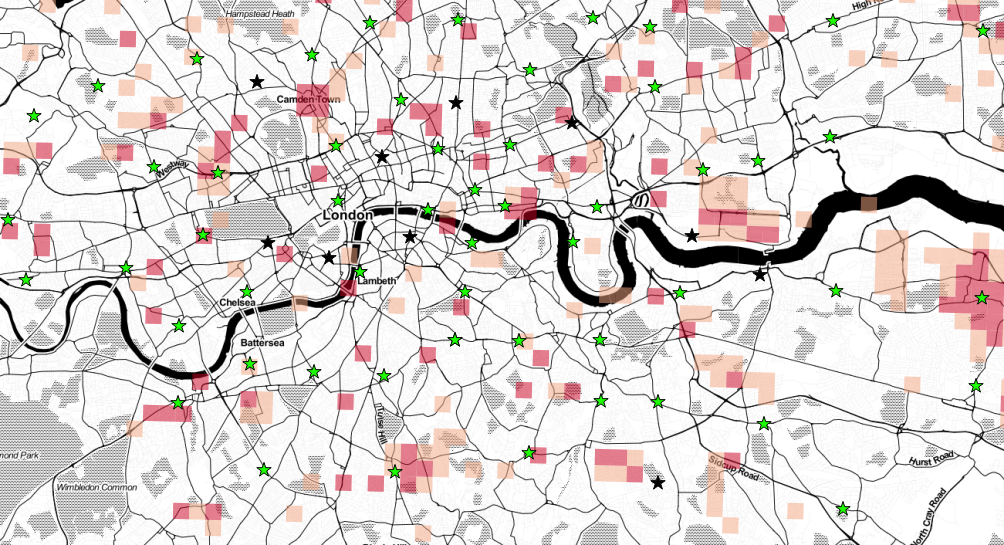
\includegraphics[width=0.74\textwidth]{figures/literature/fig_taylor_probability_2013_vs_2012.png}
\caption{Spatial probability comparisons for 2014 against 2012 (top), 2014 against 2013 (middle), and 2013 against 2012 (bottom). Red shading marks probabilities of 0.6--0.8 (light) and 0.8--1 (dark); green stars denote open stations and black stars stations closed in 2014. Source: Taylor~\cite[Fig.~8]{spatial2015}, author's manuscript. Reproduced without alteration and in the original panel order.}
\label{fig:taylor-original-closure-probabilities}
\end{figure}

\textbf{Coverage models as boundary evidence:} Service-coverage modelling for fire risk in mid-sized cities \cite{chiangrai2024} demonstrates that isochrone-based reachability analysis at multiple cut-off thresholds (3, 5, 10 minutes) can surface response-window gaps when facility locations, hazard sites, and travel-time assumptions are available. For this project, the value of that literature is mainly boundary-setting: it shows what a routing-grade coverage surface would require, while the present open-data artefact can only provide public station-address proximity and assignment-footprint context. The isochrone-surface concept itself is formalised by Andrienko and Andrienko \cite{andrienko2007} as ``a series of concentric polygons centred on a selected location, representing the areas accessible from this location within specified time budgets (e.g.\ 3, 6, 9 minutes)'' -- a definition that maps conceptually onto the LFB six-minute first-pump target but is not implemented here. Potential spatial accessibility is commonly operationalised by the two-step floating catchment area (2SFCA) method \cite{luo2003}, which combines a supplier-side service-area ratio with a demand-side aggregation under a single travel-time threshold; Luo and Wang further show that 2SFCA is a special case of the gravity model with a dichotomous travel-time impedance, exposing the artefact of binary thresholds analogous to the LFB six-minute target. 2SFCA sits within a broader landscape of accessibility measures classified by Geurs and van Wee \cite{geurs2004} along two axes -- four components (land-use, transport, temporal, individual) and four measurement perspectives (infrastructure-based, location-based, person-based, utility-based). The LFB dashboard does not implement these accessibility models because open data does not expose routing, capacity, or individual-level demand at the required granularity; instead, it keeps station-address proximity as descriptive context beside borough-level response evidence.

\textbf{Equity framing:} The framing of these spatial gaps as equity questions, rather than purely operational ones, draws on a longer urban-geography tradition. Talen and Anselin's foundational work on spatial equity \cite{talen1998} demonstrated that the choice of accessibility measure (count, gravity-based potential, average travel distance, distance-to-nearest) materially changes conclusions about whether a public service is equitably distributed -- a methodological warning that this project takes seriously by surfacing multiple aggregations (borough median, station-grouped median, hour-of-day breakdown) rather than a single composite KPI. Pereira, Schwanen and Banister \cite{pereira2017equity} update this position with a contemporary review of distributive-justice theories applied to public services: they reject horizontal equality (uniform service everywhere) as a complete equity criterion and adopt a synthesis built on Rawls' difference principle and Sen's capability approach, which requires (i) a sufficientarian floor -- a socially-defined minimum threshold of accessibility that government must guarantee -- combined with (ii) an egalitarian requirement that residual inequalities above the floor be arranged to favour the least-advantaged group. Mapped onto fire-service response, the LFB six-minute first-pump target operationalises the sufficientarian floor, while the borough- and ward-level disparities of attendance time \emph{above} that floor are the egalitarian-layer signal; the dashboard is designed to surface both layers separately rather than collapsing them into a composite KPI. Batty's commentary on big data and smart cities \cite{batty2013} argues that real-time and routinely-collected urban data are shifting urban planning's analytical horizon from years and decades toward the minutes-to-days scale on which disruptions occur, and notes that emergency-services operations research is one of the few domains already operating at this short horizon. The LFB CTRA dataset is event-tagged rather than sensor-streamed, so the analogy is partial; nevertheless, the dashboard's hour-of-day and day-of-week panels are positioned within this short-horizon framing, treating response-time variability as an operational signal rather than a long-term strategic indicator.

\subsection{Fire-Station Placement and Resource Optimisation}\label{sec:lit-optimisation}

\textbf{Covering-location lineage:} A second strand of literature applies optimisation rather than analysis. The covering-location lineage originates with the Maximal Covering Location Problem of Church and ReVelle \cite{church1974}, which formalised the trade-off between number of facilities $p$ and population covered within a service distance $S$ as a 0--1 integer program; alongside the earlier Location Set Covering Problem \cite{toregas1971}, this is the foundational pairing for emergency-service siting. Operations research models for emergency vehicle deployment have been developed continuously since the mid-1960s, spanning deterministic covering, probabilistic queueing, simulation, and dynamic relocation paradigms \cite{goldberg2004}; the present project draws on this lineage as visualisation input rather than re-solving the optimisation itself.

\textbf{Recent optimisation examples:} Recent work in this strand combines several of these threads. Bispo et al.\ \cite{reconfig2023} provide the methodologically richest example: they model Aveiro fire incidents as an inhomogeneous Poisson point process with a log-cubic predictor and population-density offset; simulate 450 realisations; cluster each via $k$-means with $k$ matched to the 27 existing fire stations to obtain candidate optimal locations; and define 90\%/99\% confidence siting regions through bivariate-normal estimation over the simulation set. Voronoi tessellation completes the layout by defining service areas. Bispo et al.\ explicitly validate the use of Euclidean distance as a road-distance proxy with $r = 0.96$, which helps justify transparent straight-line distance as a limited station-address proximity cue, not as operational coverage evidence. Multi-source geospatial optimisation work for Beijing \cite{beijing2021} integrates road network, demographic, and incident-history layers in a multi-criteria objective, and finds the city-level coverage rate falling from 96.51\% off-peak to 71.43\% at peak hours -- a time-varying coverage finding that motivates by-hour inspection while also illustrating why the present project does not claim coverage without a travel-time model. Space-syntax-augmented location-allocation models \cite{spacesyntax2023} extend the formulation by chaining maximum-coverage location-allocation with sDNA road-closeness to extend candidate points to buildable regions, motivated by the empirical observation that approximately 60\% of fire-department tasks are technical rescues rather than fire suppression -- a category imbalance that maps directly onto the LFB's 46.5\%/40.6\%/12.9\% (false alarm / special service / fire) split. Bolouri et al.\ \cite{ocmola2018} extend this strand by combining three objectives -- minimising demand-to-station distance, minimising travel time, and maximising five-minute coverage -- under explicit station-capacity and ordered-priority constraints, solved by genetic-algorithm and simulated-annealing benchmarks on Tehran's Region~11.

\textbf{Boundary for this project:} These papers share a common limitation from the present project's perspective: they produce a static optimisation output (even when, as in Bispo et al., that output includes confidence regions and multiple strategy classes), not an interactive evidence-inspection surface. The present project deliberately does \emph{not} attempt to solve the location-allocation problem; instead, it provides a visual-analytics surface on which users can compare empirical response-time gaps with station-related context while leaving any optimisation or reconfiguration judgement outside the artefact. This positions the project as complementary to, rather than competing with, the optimisation literature: an external optimisation pipeline could supply candidate layouts for a validated operational study, and the dashboard pattern would then help planners inspect consequences under explicitly stated assumptions.

\subsection{LFB-Specific Prior Work}\label{sec:lit-lfb}

The most directly comparable analysis is Yang and Benidir~\cite{antoyang2020}, who regress borough fire counts on thirteen socio-economic features and report $R^2=0.90$ for a six-variable specification. It shows that borough demand relates to population and deprivation context, but it is a static, pre-2024 modelling exercise. This project does not reproduce that regression because its implemented data contract contains no socio-economic predictors; the study instead marks a future contextual-analysis route and a contrast with the present descriptive, uncertainty-aware interface.

Two earlier public-facing LFB artefacts sharpen the comparison. The GOV.UK prototype combines a ward/borough choropleth with response-time and daily breakdowns~\cite{govuk2014}; the ODI map lets users toggle ten proposed station closures and inspect modelled borough impacts~\cite{odi2013}. Both demonstrate demand for interactive public evidence, but use pre-2014 data and neither presents the current project's recorded-time denominator, coordinate-completeness field, or matched-mobilisation qualifier. The contribution here is therefore not the first LFB map, but a current and reproducible linked evidence package with these caveats carried alongside the result.

\subsection{Predictive Analytics}\label{sec:lit-predictive}

Sharma et al.~\cite{predictive2024} build Negative-Binomial event-count models for 402 Edmonton neighbourhoods and 30 station service areas, with Conditional Random Forest feature pre-selection. Neighbourhood total-count prediction is feasible (weekly MAE 0.81 against a mean of 2.06), but event-type prediction is undermined by zero inflation and requires coarser aggregation. Post-COVID errors also differ sharply by event type. These findings justify the present borough-scale descriptive design and caution against adding an under-supported forecasting model merely for technical breadth; predictive modelling remains an alternative, not an implemented component.

\subsection{Synthesis and Identified Gap}\label{sec:lit-synthesis}

Table~\ref{tab:litsynth} summarises the seven literature strands against how each is used in this project. Reading across these strands reveals three patterns that no single paper makes visible on its own, and which jointly motivate the present project's positioning.

\textbf{Pattern 1: Spatial heterogeneity is universally reported but uncertainty is rarely visualised.} Park et al.\ \cite{seoul2024}, Taylor \cite{spatial2015}, Bispo et al.\ \cite{reconfig2023}, Wang et al.\ \cite{beijing2021}, Tian et al.\ \cite{spacesyntax2023}, and Bolouri et al.\ \cite{ocmola2018} all surface spatial heterogeneity in incident density or response time at sub-city granularity. Yet none of these papers \emph{visualises} the uncertainty in its estimates: Taylor's 80\% posterior probability is rendered as a binary ``concerning'' tag rather than a continuous credibility surface; Bispo et al.\ produce 90\%/99\% siting-confidence ellipses but a single static map; Park et al.\ render Moran's $I$ as a single point estimate without dispersion. The literatures Hullman et al.\ \cite{hullman2015hops}, MacEachren et al.\ \cite{maceachren2012} and Padilla et al.\ \cite{padilla2018} diagnose for general InfoVis -- that point-estimate displays systematically mislead non-expert decision-makers -- have not yet been applied to fire-service performance data. The present dashboard and report make a first, bounded attempt to close that gap through median-to-p95 distribution ranges, denominator exposure, precise-coordinate coverage fields, and explicit second-iteration commitments for fuller uncertainty encodings.

\textbf{Pattern 2: Optimisation outputs are static; decision contexts are scenario-driven.} Bispo et al., Wang et al., Bolouri et al., Tian et al., and the OR survey of Goldberg \cite{goldberg2004} all produce static optimisation outputs -- even when, as in Bispo et al., that output includes confidence regions and multiple strategy classes. The actual decision context, however, is inherently interactive: a fire chief weighing a station closure against political feasibility, budget, and public acceptance needs to compare scenarios under their own assumptions, not consume a single ``optimal'' layout. The dashboard genres of Sarikaya et al.\ \cite{sarikaya2018} and the design patterns of Bach et al.\ \cite{bach2023patterns} both name interactive scenario exploration as an under-served pattern; Pereira, Schwanen and Banister \cite{pereira2017equity} make the political-philosophy point complementary: an automated optimum can satisfy aggregate utility while violating distributive-justice constraints that only a deliberative process can specify. The present project deliberately occupies that interactive scenario-exploration role rather than competing on optimisation rigour.

\textbf{Pattern 3: Sufficientarian thresholds and egalitarian distribution are conflated.} Park et al.'s 5-minute Seoul threshold and the LFB's 6-minute first-pump target are both rendered as \emph{sufficientarian} floors, but the optimisation literature reports binary ``coverage'' against those floors and rarely discusses within-threshold variance. Pereira et al.\ \cite{pereira2017equity} argue, drawing on Rawls and Sen, that distributive justice in public services demands \emph{both} a sufficientarian floor \emph{and} egalitarian distribution above it; horizontal equality (uniform service) is a category-coarse target that can mask group-level disparities. No reviewed paper combines both layers of evaluation. The design decision to surface ``\% of incidents above the 6-minute target'' and ``borough-level distribution of attendance time below the target'' in the dashboard's linked panels, rather than as a single ranking, operationalises that two-layer view directly.

\begin{table}[h]
\centering
\footnotesize
\begin{tabularx}{\textwidth}{p{3.2cm}p{3cm}X}
\toprule
Strand & Method & How used here \\
\midrule
VA design \& dashboards & Mantra; nested model; pattern catalogues & Dashboard interaction structure; design-language anchor; WP4 plan \\
Uncertainty visualisation & HOPs; visual-semiotics; cognitive framework & Median--p95 ranges and coverage exposure now; quantile/fuzziness/natural-frequency encodings as second-iteration targets \\
VA for emergency mgmt & Linked map / time views & Three-pane layout, linked brushing \\
Spatial response-time modelling & Hazard models on LFB data & Equity framing; 2014 closure anchor \\
Location-allocation optimisation & Mixed-integer / point-process & Informs the proxy; not an optimisation engine \\
LFB-specific prior work & Static regression, blog dashboards & Borough benchmark for descriptive views \\
Spatial equity / smart cities & Accessibility; Rawls + capability approach & Sufficientarian floor + egalitarian layer; short-horizon framing \\
Predictive analytics & NB regression + CRF & Justifies VA-not-prediction choice; post-COVID baseline caveat \\
\bottomrule
\end{tabularx}
\caption{Literature strands and how each informs this project.}
\label{tab:litsynth}
\end{table}

Two methodological choices warrant justification. First, visual analytics was selected over predictive modelling along the lines of \cite{predictive2024} because the intended user is exploring where response-time gaps are and where the data is too incomplete to trust, not forecasting next month's incident count; Hullman et al.\ \cite{hullman2015hops} document how single-point predictions are systematically mis-read as deterministic. Second, exploratory station-related context was selected over location-allocation optimisation as in \cite{ocmola2018,beijing2021,reconfig2023} because a real optimisation needs routing, dispatch rules, and station capacity, none of which LFB open data exposes at the right granularity. A black-box ``optimal layout'' would too easily be read as a relocation recommendation, which the station-context framing and the distributive-justice constraints articulated by \cite{pereira2017equity} both argue against.

The project therefore focuses on a practical problem in the LFB data: how to let users explore borough-level response-time gaps while still seeing where the spatial evidence is incomplete. It builds this as an \textbf{uncertainty-aware visual-analytics interface} for emergency-service response equity. The linked-view layout is drawn from PanViz, the borough-level response framing from Park et al., the 2014 closure-cohort comparison from \cite{spatial2015}, and the two-layer equity-evaluation logic from \cite{pereira2017equity}. The 62\% missing-coordinate share is treated as something the user should see in the interface and report-side evidence, rather than as a preprocessing assumption to be hidden. The 2014 closure cohort is used as a historical anchor for response-time geography, not as a claim that those closures alone explain what we see in 2024--2026; intervening changes in population, traffic, and service organisation are acknowledged.
